\section{Протекание сухого электронно-лучевого травления при экспонировании по произвольной области}

Приведенные выше промоделированные профили относятся к структурам, получаемым методом СЭЛТР при экспонировании вдоль серии параллельных линий либо вдоль одиночной линии.
Однако, при моделировании может быть заложено произвольное распределение плотности тока по области экспонирования.
Для демонстрации возможностей алгоритма были промоделированы профили, получаемые при экспонировании электронным лучом, плотность тока в котором описывается суммой двух (рисунок~\ref{fig:DEBER_multibeam} a)) или четырех (рисунок~\ref{fig:DEBER_multibeam}~б)) функций Гаусса.
За счет этого разработанные в данной работе модель СЭЛТР и алгоритм моделирования профиля линии, получаемой в этом процессе, могут использоваться при определении параметров для формирования методом СЭЛТР необходимого профиля.
В самом деле, для получения методом СЭЛТР рельефа, профиль которого согласуется с предельным разрешением метода, параметры экспонирования и последующего охлаждения образца могут быть подобраны путем многократного моделирования конечного профиля с учетом выявленных характерных особенностей метода.

\begin{figure}[t!]
	\begin{minipage}{0.48\textwidth}
%		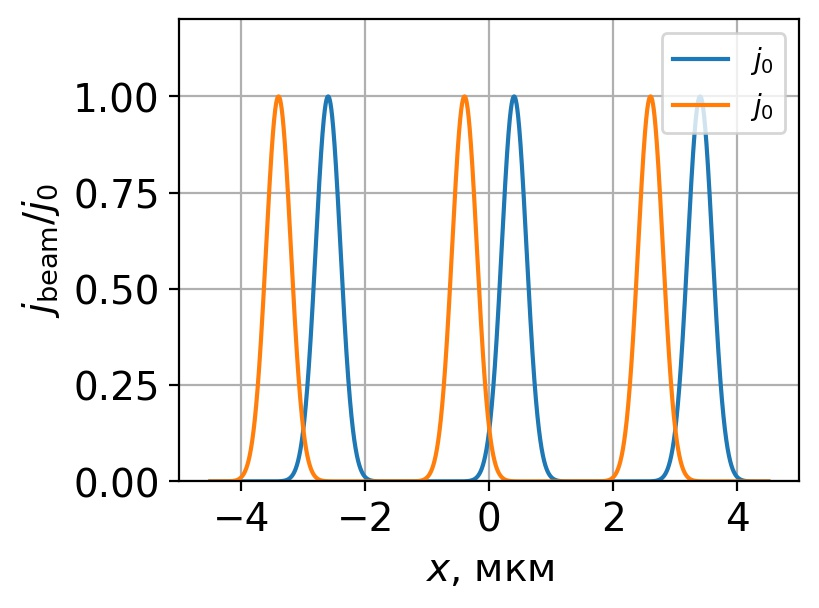
\includegraphics[width=\linewidth]{DEBER_asymmetric/pm_400_colors_200} \\
		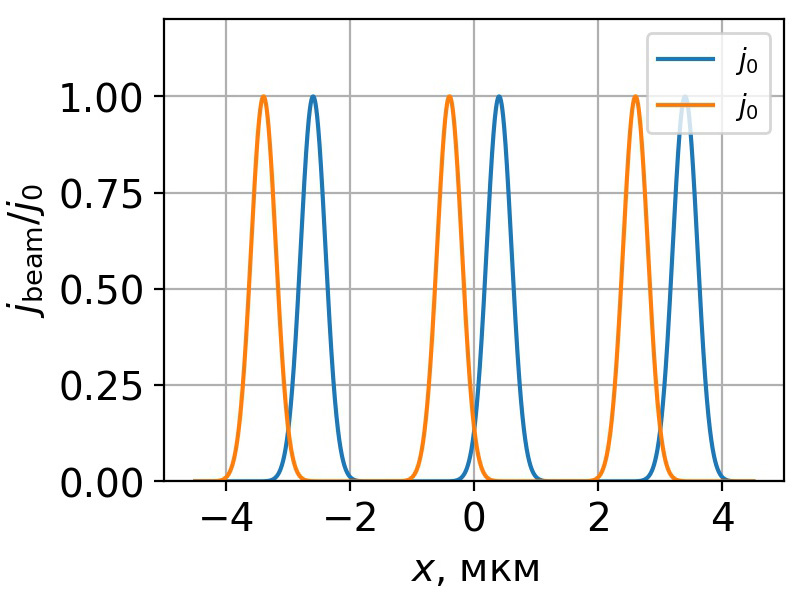
\includegraphics[width=\linewidth]{DEBER_asymmetric/pm_400_colors_200_cut} \\
		\vspace{-13em} \\ \text{\hspace{0em} a}) \\ \vspace{13em}
	\end{minipage}
	\begin{minipage}{0.48\textwidth}
		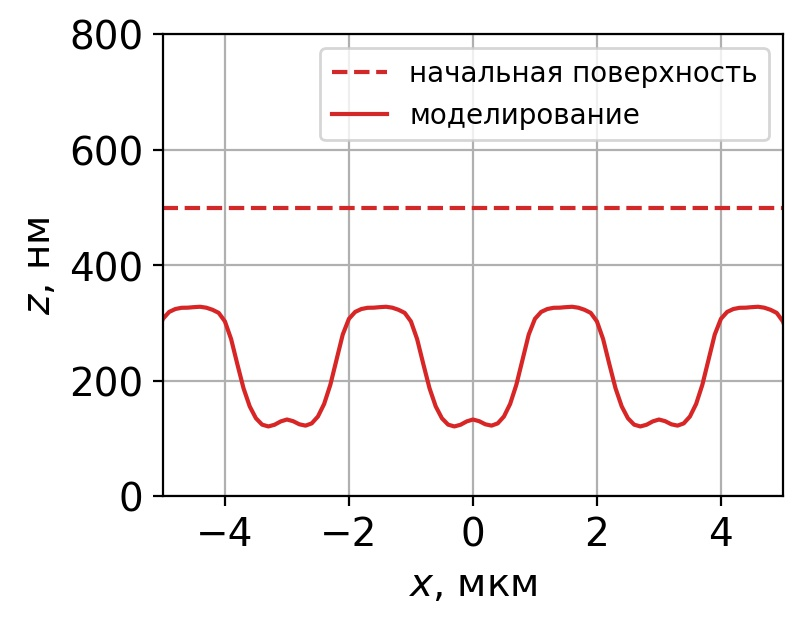
\includegraphics[width=\linewidth]{DEBER_asymmetric/pm_400_200} \\
		\vspace{-13em} \\ \text{\hspace{-0.1em} б}) \\ \vspace{13em}
	\end{minipage}
	
	\vspace{-3em}
	
	\begin{minipage}{0.48\textwidth}
		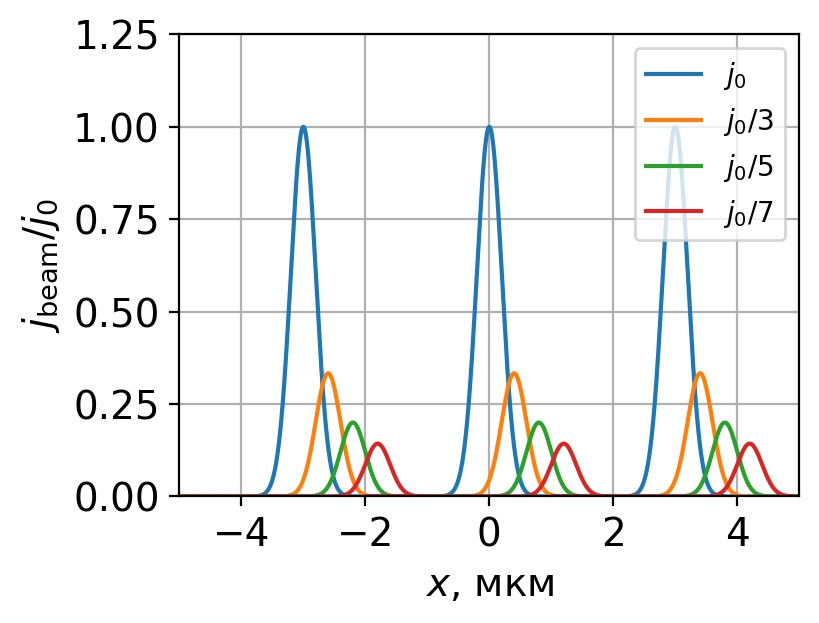
\includegraphics[width=\linewidth]{DEBER_asymmetric/asymmetric_beam_200} \\
		\vspace{-13em} \\ \text{\hspace{0em} в}) \\ \vspace{13em}
	\end{minipage}
	\begin{minipage}{0.48\textwidth}
		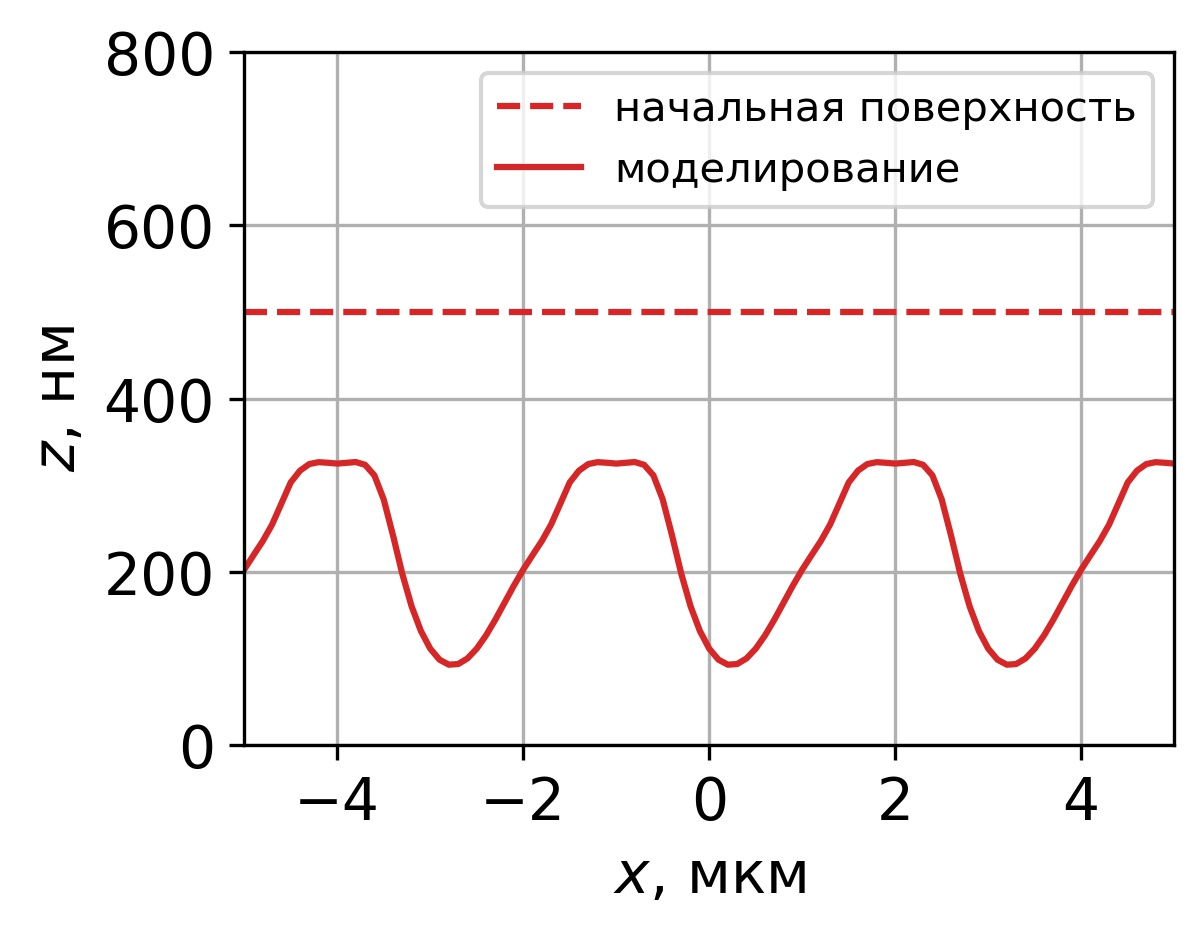
\includegraphics[width=\linewidth]{DEBER_asymmetric/asymmetric_profile_200} \\
		\vspace{-13em} \\ \text{\hspace{-0.1em} г}) \\ \vspace{13em}
	\end{minipage}
	\vspace{-3em}
	\caption{Промоделированные периодические профили с периодом 3~мкм, полученные в слое ПММА с начальной толщиной 500 нм методом СЭЛТР при экспонировании по области для двух различных распределений плотности тока в пучке. Температура резиста при экспонировании -- 150 $^\circ$C/с, время экспонирования -- 100 с, ток экспонирования -- 4.56 нА. Экспонирование резиста производится ``в кадр'' с параметрами кадра, описанными в разделе~\ref{sec:verification}. Охлаждение производится в соответствии с кривой охлаждения, приведенной на рисунке~\ref{fig:exp_cooling}.}
	\label{fig:DEBER_multibeam}
\end{figure}
